\section{Design Patterns}
\subsection{Model View ViewModel (MVVM) Pattern}
\begin{figure}[H]
	\centering
	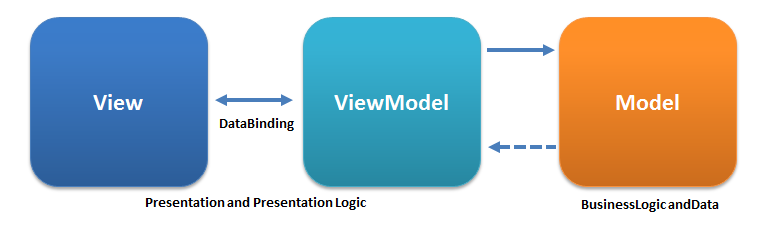
\includegraphics[scale=0.6]{Figures/WebImages/MVVMPattern}\\
	\caption{The MVVM Pattern - http://en.wikipedia.org/wiki/Model\_View\_ViewModel}
	\label{fig:MVVMPattern}
\end{figure}
The \texttt{DriveIT Windows Client} uses the \emph{Model View ViewModel} architectural pattern which tries to ensure a clear separation between the model and the view. The pattern derives from both the \emph{Model View Controller} pattern and the \emph{Presentation Model} design pattern and therefore has some of the same attributes. By using the MVVM pattern we created a more testable and easier expandable application.

Furthermore we used \emph{Microsoft Blend}'s \emph{Behavior Actions} to encapsulate calls and commands from the View such that View elements would not get send to the ViewModel. These actions are implemented to ensure low coupling.\\

A build in part of \textit{Model View ViewModel} is a version of the Observer-Pattern. This is done by creating data-binding between the View and their ViewModel. In WPF this is achieved by having the viewmodels implement the interface \texttt{INotifyPropertyChanged} which will notify the view when the ViewModel has changed. By using this interface the ViewModel knows nothing of the View and cannot directly change its attributes.

\subsection{Adapter Pattern}
The \texttt{DriveIT Windows Client} uses the \textit{Model View ViewModel} architectural pattern which tries to ensure a clear separation between the model and the view. The pattern derives from both the \textit{Model View Controller} pattern and the \textit{Presentation Model} design pattern and therefore has some of the same attributes. By using the MVVM pattern we created a more testable and easier expandable application. Furthermore we used \textit{Microsoft Blend}'s \textit{Behavior Actions} to encapsulate calls and commands from the View such that View elements would not get send to the ViewModel. These actions are implemented to ensure low coupling.\\


\subsection{Adapter Pattern}
The \textit{Adapter pattern} allows the coder to encapsulate an object its methods and properties in an "Adapter" class. Since the \texttt{DriveIT Windows Client} uses the MVVM design pattern, and The \texttt{DriveIT Web API} uses Data Transfer Objects(DTO) to send and receive data and DTO's are only meant to transfer data, an Adapter Pattern fits perfectly. All Single Entitiy ViewModels in the \texttt{DriveIT.WindowsClient.ViewModels} name-space functions as Adapters for their corresponding DTO. E.g The CarViewModel class is an adapter for the CarDto class.\\ 

This implementation provides the \texttt{DriveIT Windows Client} with an easy way to manipulate data, while still retaining the data-structure such that entities can be Created, Read, Updated and Deleted over the \texttt{DriveIT Web API} without the having to convert Client Classes to API Classes.

\subsection{Model View Controller (MVC) Pattern}
\begin{figure}[H]
	\centering
	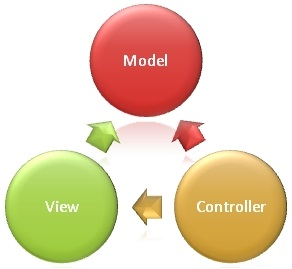
\includegraphics[scale=0.6]{Figures/WebImages/MVCPattern}\\
	\caption{The MVC Pattern - http://www.w3schools.com/aspnet/mvc_intro.asp}
	\label{fig:MVCPattern}
\end{figure}
The \texttt{DriveIT Web Client} uses the "Model View Controller" architectural pattern, which is making a seperation of the business logic (model) and the input control (controller) from the display logic (view).

The model is the part of the application that wil be handling all the logic for the application data. The models are being used to store data from the dabatase.
The view is the part of the application that will be handling the representation of the data. Most often, this data will be given by the model.
The controller is the part of the application that will be handling the user interaction with the \texttt{DriveIT Web Client}. The controllers reads the user input and updates the model's state.

The MVC pattern allows for seperation of the model, view and the controller classes, such that their individual purposes are clearly distinct from each other. This means that different developers are able to work on each of the individual parts of the MVC pattern, E.g we are able to work on the view without depending on the business logic (model) or the input (controller). By making this distinction between different parts of the MVC pattern, it also makes it easier to test our \texttt{DriveIT Web Client} application, and remain a good data-structure throughout the development of our Web Client.

\todo{Write more specific about how we have implemented it in our system.}

\subsection{Façade Pattern}
The facade design pattern is used several times in the \texttt{DriveIT System}.
The \texttt{Persistent Storage} sub system uses a facade pattern do hide the internal sub systems that accomplish the functionality defined in the \texttt{IPersistentStorage} interface.

The \texttt{DriveITContext} defined in the sub system is used by an implementer, \texttt{EntityStorage}, on the interface, but is hidden for users of the interface. 

\begin{figure}[H]
	\centering
	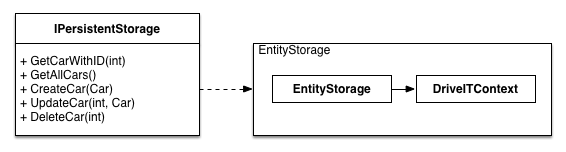
\includegraphics[scale=0.6]{Figures/FacadePatternPersistentStorage}\\
	% place the figure in the Figures folder (located with the main file)
	% you need to fix the scale a few times to get it right, but latex does not compress so one can always zoom in to see details.
	\caption{The Facade Pattern of IPersistentStorage.}
	\label{fig:The Facade Pattern of IPersistentStorage.}
	% label it something meanfull
\end{figure}

\begin{figure}[H]
	\centering
	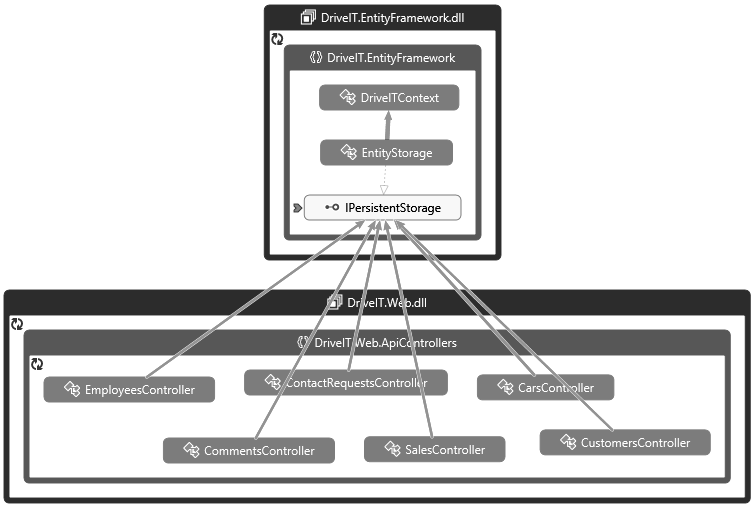
\includegraphics[scale=0.6]{Figures/FacadeKindOfPattern}\\
	% place the figure in the Figures folder (located with the main file)
	% you need to fix the scale a few times to get it right, but latex does not compress so one can always zoom in to see details.
	\caption{The Facade Pattern Used by the \texttt{DriveIT Web API}.}
	\label{fig:The Facade Pattern Used by the DriveIT Web API.}
	% label it something meanfull
\end{figure}
